\documentclass{beamer}
\usepackage{default}
\usepackage[utf8]{inputenc}
\usepackage[french]{babel}
\uselanguage{French}
\languagepath{French}
\usetheme{Antibes}

\title{Introduction à ROS}

\author{Maxime St-Pierre}

\institute{Walking Machine - ÉTS}

\date{16 septembre 2017}

\begin{document}

\begin{frame}
\titlepage
\end{frame}

\begin{frame}
\frametitle{Table des matières}
\tableofcontents

\end{frame}

\section{Historique}

\begin{frame}{Historique}
\begin{columns}
	\column{0.5\textwidth}
	\begin{itemize}
		\item Crée en 2007 par des anciens de Stanford
		\item Developpement continuer chez Willow Garage de 2008 a 2013
		\item Création de Open Source Robotics Foundation pour continuer le developpement.
	\end{itemize}

	\column{0.5\textwidth}
	
\includegraphics[width=\textwidth]{ros_logo.png}
\end{columns}
\end{frame}

\section{Ses quoi ROS}
\begin{frame}{Ses quoi ROS}
\begin{itemize}
	\item ROS veux dire Robot Operating System
	\begin{itemize}
		\item Même si le nom veux dire que ses un système d'explotation ce n'est pas un.
		\item Ses un Middleware pour aider la réutilisation de code.
	\end{itemize}
	\item Fonctionne sur le principe de publisher subscriber.
\end{itemize}
\end{frame}

\begin{frame}{Robot qui utilise ROS}
\begin{columns}
	\column{0.5\textwidth}
	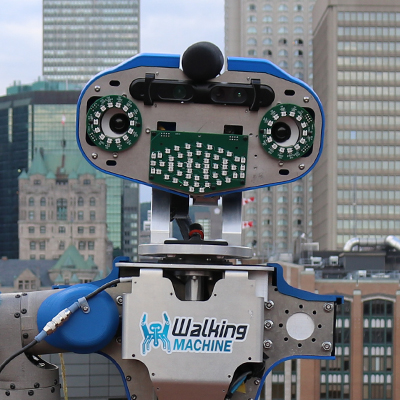
\includegraphics[width=\textwidth]{sara.jpg}
	
	\column{0.5\textwidth}
	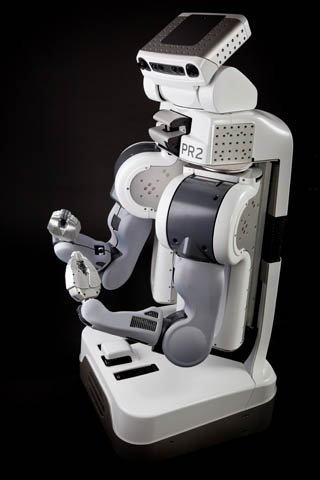
\includegraphics[width=\textwidth]{PR2.jpg}
\end{columns}
\end{frame}

\section{Pourquoi utiliser ROS}

\begin{frame}{Pourquoi utiliser ROS}
	\begin{itemize}
		\item Outil déja préfaite
		\item Grande communauté
		\item Plusieurs chercheure developpe des packages pour diverses hardware.
	\end{itemize}
\end{frame}

\section{La base de ROS}

\begin{frame}{La base de ROS}
Les principes de base de ROS sont:
\begin{itemize}
\end{itemize}
\end{frame}
\end{document}

